\documentclass[11pt, letterpaper]{article}

% Fonts and Encoding
\usepackage[utf8]{inputenc}
\usepackage[T1]{fontenc}
\usepackage{lmodern} % High-quality Latin Modern vector font

% Math and Symbols
\usepackage{amsmath, amssymb, amsthm, amsfonts, mathrsfs, mathtools}

% Layout and Geometry
\usepackage{geometry}
\geometry{letterpaper, margin=1in}
\setlength{\parindent}{0pt}
\setlength{\parskip}{0.6em}

% Formatting and Graphics
\usepackage{graphicx, xcolor, enumitem, booktabs, array, tabularx}

% TikZ for Illustrations
\usepackage{tikz}
\usetikzlibrary{arrows.meta, positioning, shapes.geometric, calc, backgrounds, matrix}

% Clickable Links and TOC
\usepackage{hyperref}
\hypersetup{
    colorlinks=true,
    linkcolor=blue,
    filecolor=magenta,      
    urlcolor=cyan,
    pdftitle={Advanced Mathematics Topic},
}

% Theorem Environments
\newtheorem{theorem}{Theorem}[section]
\newtheorem{lemma}[theorem]{Lemma}
\newtheorem{proposition}[theorem]{Proposition}
\newtheorem{corollary}[theorem]{Corollary}
\theoremstyle{definition}
\newtheorem{definition}{Definition}[section]
\newtheorem{axiom}{Axiom}[section]
\newtheorem{example}{Example}[section]
\theoremstyle{remark}
\newtheorem{remark}{Remark}[section]

% Custom Commands (Enforced standard notation)
\newcommand{\R}{\mathbb{R}}
\newcommand{\N}{\mathbb{N}}
\newcommand{\Z}{\mathbb{Z}}
\newcommand{\Q}{\mathbb{Q}}
\newcommand{\E}{\mathbb{E}}
\newcommand{\Prob}{\mathbb{P}}
\newcommand{\F}{\mathcal{F}}

\begin{document}

\title{\textbf{Mastering the Singular Value Decomposition (SVD)}}
\author{Tashfeen Omran}
\date{\today}
\maketitle

\tableofcontents
\newpage

\section{Part 1: Comprehensive Introduction, Context, and Prerequisites}

\subsection{Core Concepts}
The Singular Value Decomposition (SVD) is arguably the most fundamental and universally applicable matrix factorization in applied linear algebra. While diagonalization ($A = PDP^{-1}$) is restricted to square matrices with a full set of eigenvectors, and orthogonal diagonalization ($A = PDP^T$) is restricted to symmetric matrices, the SVD can be applied to \textbf{any} $m \times n$ matrix $A$. 

The SVD factors an $m \times n$ matrix $A$ into the product of three matrices:
\[ A = U \Sigma V^T \]
where:
\begin{itemize}
    \item $U$ is an $m \times m$ orthogonal matrix. Its columns are called the \textbf{left singular vectors} of $A$.
    \item $\Sigma$ is an $m \times n$ ``diagonal'' matrix containing the \textbf{singular values} of $A$, denoted by $\sigma_i$, arranged in descending order ($\sigma_1 \geq \sigma_2 \geq \dots \geq \sigma_r > 0$).
    \item $V$ is an $n \times n$ orthogonal matrix. Its columns are called the \textbf{right singular vectors} of $A$.
\end{itemize}

\subsection{Intuition and Derivation}
Geometrically, the SVD states that any linear transformation $x \mapsto Ax$ can be decomposed into three fundamental geometric actions:
1. A rotation or reflection in the domain space (multiplication by $V^T$).
2. An independent scaling along the coordinate axes (multiplication by $\Sigma$).
3. A final rotation or reflection in the target space (multiplication by $U$).

To derive this, we look at the matrix $A^TA$. Regardless of $A$, the matrix $A^TA$ is always a symmetric $n \times n$ matrix. By the Spectral Theorem, $A^TA$ can be orthogonally diagonalized. Its eigenvalues $\lambda_i$ are always non-negative. The singular values of $A$ are defined as the square roots of these eigenvalues: $\sigma_i = \sqrt{\lambda_i}$. The orthonormal eigenvectors of $A^TA$ form the matrix $V$. The columns of $U$ are then constructed by mapping the basis vectors $v_i$ through $A$ and normalizing them: $u_i = \frac{1}{\sigma_i}Av_i$.

\subsection{Historical Context and Motivation}
The SVD was independently developed by Eugenio Beltrami (1873) and Camille Jordan (1874) for real square matrices, and later extended to complex matrices by Autonne (1902) and to general rectangular matrices by Eckart and Young (1936). The primary mathematical motivation was to find a way to approximate a complex, high-dimensional matrix with a simpler, lower-rank matrix. Today, this Eckart-Young-Mirsky theorem forms the backbone of data compression and principal component analysis.

\subsection{Key Formulas}
\begin{itemize}
    \item \textbf{Singular Values:} $\sigma_i = \sqrt{\lambda_i}$, where $\lambda_i$ are the eigenvalues of $A^TA$.
    \item \textbf{Right Singular Vectors ($v_i$):} The orthonormal eigenvectors of $A^TA$.
    \item \textbf{Left Singular Vectors ($u_i$):} $u_i = \frac{1}{\sigma_i} A v_i$ for $\sigma_i > 0$.
    \item \textbf{Spectral Decomposition of A:} $A = \sigma_1 u_1 v_1^T + \sigma_2 u_2 v_2^T + \dots + \sigma_r u_r v_r^T$.
\end{itemize}

\subsection{Prerequisites}
To master this topic, you must be proficient in:
1. Finding eigenvalues and eigenvectors (solving $\det(A - \lambda I) = 0$).
2. Orthogonal diagonalization of symmetric matrices.
3. The Gram-Schmidt process (for extending orthonormal bases).
4. Matrix multiplication and transpose properties (e.g., $(AB)^T = B^T A^T$).

\newpage
\section{Part 2: Detailed Homework Solutions}
\textit{Note: Following strategic selection protocols, we have selected a representative set of problems that cover every distinct archetype present in the provided text, ensuring comprehensive mastery without redundant repetition.}

\subsection{Problem 1: Finding Singular Values}
\textbf{Problem:} Find the singular values of the matrix $A = \begin{bmatrix} 1 & 0 \\ 0 & -3 \end{bmatrix}$.

\textbf{Solution:}
Step 1: Compute $A^TA$.
\[
A^TA = \begin{bmatrix} 1 & 0 \\ 0 & -3 \end{bmatrix} \begin{bmatrix} 1 & 0 \\ 0 & -3 \end{bmatrix} = \begin{bmatrix} 1 & 0 \\ 0 & 9 \end{bmatrix}
\]
Step 2: Find the eigenvalues of $A^TA$.
Since $A^TA$ is a diagonal matrix, its eigenvalues are simply its diagonal entries.
\[
\lambda_1 = 9, \quad \lambda_2 = 1
\]
Step 3: Compute the singular values.
The singular values $\sigma_i$ are the square roots of the eigenvalues, arranged in decreasing order.
\[
\sigma_1 = \sqrt{9} = 3, \quad \sigma_2 = \sqrt{1} = 1
\]
\textbf{Final Answer:} The singular values are $\sigma_1 = 3$ and $\sigma_2 = 1$.

\vspace{1em}
\subsection{Problem 3: Finding Singular Values of an Upper Triangular Matrix}
\textbf{Problem:} Find the singular values of the matrix $A = \begin{bmatrix} 2 & 3 \\ 0 & 2 \end{bmatrix}$.

\textbf{Solution:}
Step 1: Compute $A^TA$.
\[
A^TA = \begin{bmatrix} 2 & 0 \\ 3 & 2 \end{bmatrix} \begin{bmatrix} 2 & 3 \\ 0 & 2 \end{bmatrix} = \begin{bmatrix} 4 & 6 \\ 6 & 13 \end{bmatrix}
\]
Step 2: Find the eigenvalues of $A^TA$.
We solve the characteristic equation $\det(A^TA - \lambda I) = 0$:
\[
\det \begin{bmatrix} 4 - \lambda & 6 \\ 6 & 13 - \lambda \end{bmatrix} = (4 - \lambda)(13 - \lambda) - 36 = 0
\]
\[
52 - 4\lambda - 13\lambda + \lambda^2 - 36 = 0 \implies \lambda^2 - 17\lambda + 16 = 0
\]
Factoring the quadratic:
\[
(\lambda - 16)(\lambda - 1) = 0 \implies \lambda_1 = 16, \quad \lambda_2 = 1
\]
Step 3: Compute the singular values.
\[
\sigma_1 = \sqrt{16} = 4, \quad \sigma_2 = \sqrt{1} = 1
\]
\textbf{Final Answer:} The singular values are $\sigma_1 = 4$ and $\sigma_2 = 1$.

\vspace{1em}
\subsection{Problem 5: Constructing an SVD}
\textbf{Problem:} Find an SVD of the matrix $A = \begin{bmatrix} -2 & 0 \\ 0 & 0 \end{bmatrix}$.

\textbf{Solution:}
Step 1: Compute $A^TA$ and its eigenvalues/eigenvectors.
\[
A^TA = \begin{bmatrix} -2 & 0 \\ 0 & 0 \end{bmatrix} \begin{bmatrix} -2 & 0 \\ 0 & 0 \end{bmatrix} = \begin{bmatrix} 4 & 0 \\ 0 & 0 \end{bmatrix}
\]
The eigenvalues are $\lambda_1 = 4$ and $\lambda_2 = 0$. The corresponding orthonormal eigenvectors are the standard basis vectors:
\[
v_1 = \begin{bmatrix} 1 \\ 0 \end{bmatrix}, \quad v_2 = \begin{bmatrix} 0 \\ 1 \end{bmatrix}
\]
Thus, the matrix $V$ is:
\[
V = \begin{bmatrix} 1 & 0 \\ 0 & 1 \end{bmatrix}
\]
Step 2: Set up $\Sigma$.
The singular values are $\sigma_1 = \sqrt{4} = 2$ and $\sigma_2 = 0$.
\[
\Sigma = \begin{bmatrix} 2 & 0 \\ 0 & 0 \end{bmatrix}
\]
Step 3: Construct $U$.
We find the first column of $U$ using $u_1 = \frac{1}{\sigma_1} A v_1$:
\[
u_1 = \frac{1}{2} \begin{bmatrix} -2 & 0 \\ 0 & 0 \end{bmatrix} \begin{bmatrix} 1 \\ 0 \end{bmatrix} = \frac{1}{2} \begin{bmatrix} -2 \\ 0 \end{bmatrix} = \begin{bmatrix} -1 \\ 0 \end{bmatrix}
\]
Since $A$ is $2 \times 2$, $U$ must be a $2 \times 2$ orthogonal matrix. We need a unit vector $u_2$ orthogonal to $u_1$. By inspection, $u_2 = \begin{bmatrix} 0 \\ 1 \end{bmatrix}$ works perfectly.
\[
U = \begin{bmatrix} -1 & 0 \\ 0 & 1 \end{bmatrix}
\]
\textbf{Final Answer:} $A = U \Sigma V^T = \begin{bmatrix} -1 & 0 \\ 0 & 1 \end{bmatrix} \begin{bmatrix} 2 & 0 \\ 0 & 0 \end{bmatrix} \begin{bmatrix} 1 & 0 \\ 0 & 1 \end{bmatrix}$.

\vspace{1em}
\subsection{Problem 7: SVD of a Full-Rank $2 \times 2$ Matrix}
\textbf{Problem:} Find an SVD of $A = \begin{bmatrix} 2 & -1 \\ 2 & 2 \end{bmatrix}$.

\textbf{Solution:}
Step 1: Compute $A^TA$.
\[
A^TA = \begin{bmatrix} 2 & 2 \\ -1 & 2 \end{bmatrix} \begin{bmatrix} 2 & -1 \\ 2 & 2 \end{bmatrix} = \begin{bmatrix} 8 & 2 \\ 2 & 5 \end{bmatrix}
\]
Step 2: Find eigenvalues of $A^TA$.
\[
\det \begin{bmatrix} 8 - \lambda & 2 \\ 2 & 5 - \lambda \end{bmatrix} = (8 - \lambda)(5 - \lambda) - 4 = \lambda^2 - 13\lambda + 36 = 0
\]
\[
(\lambda - 9)(\lambda - 4) = 0 \implies \lambda_1 = 9, \quad \lambda_2 = 4
\]
The singular values are $\sigma_1 = 3$ and $\sigma_2 = 2$. Thus, $\Sigma = \begin{bmatrix} 3 & 0 \\ 0 & 2 \end{bmatrix}$.

Step 3: Find orthonormal eigenvectors for $V$.
For $\lambda_1 = 9$:
\[
A^TA - 9I = \begin{bmatrix} -1 & 2 \\ 2 & -4 \end{bmatrix} \implies -x_1 + 2x_2 = 0 \implies x_1 = 2x_2
\]
A basis vector is $\begin{bmatrix} 2 \\ 1 \end{bmatrix}$. Normalizing gives $v_1 = \frac{1}{\sqrt{5}}\begin{bmatrix} 2 \\ 1 \end{bmatrix}$.

For $\lambda_2 = 4$:
\[
A^TA - 4I = \begin{bmatrix} 4 & 2 \\ 2 & 1 \end{bmatrix} \implies 2x_1 + x_2 = 0 \implies x_2 = -2x_1
\]
A basis vector is $\begin{bmatrix} -1 \\ 2 \end{bmatrix}$. Normalizing gives $v_2 = \frac{1}{\sqrt{5}}\begin{bmatrix} -1 \\ 2 \end{bmatrix}$.
\[
V = \frac{1}{\sqrt{5}} \begin{bmatrix} 2 & -1 \\ 1 & 2 \end{bmatrix}
\]

Step 4: Construct $U$.
\[
u_1 = \frac{1}{\sigma_1} A v_1 = \frac{1}{3} \begin{bmatrix} 2 & -1 \\ 2 & 2 \end{bmatrix} \left( \frac{1}{\sqrt{5}} \begin{bmatrix} 2 \\ 1 \end{bmatrix} \right) = \frac{1}{3\sqrt{5}} \begin{bmatrix} 3 \\ 6 \end{bmatrix} = \frac{1}{\sqrt{5}} \begin{bmatrix} 1 \\ 2 \end{bmatrix}
\]
\[
u_2 = \frac{1}{\sigma_2} A v_2 = \frac{1}{2} \begin{bmatrix} 2 & -1 \\ 2 & 2 \end{bmatrix} \left( \frac{1}{\sqrt{5}} \begin{bmatrix} -1 \\ 2 \end{bmatrix} \right) = \frac{1}{2\sqrt{5}} \begin{bmatrix} -4 \\ 2 \end{bmatrix} = \frac{1}{\sqrt{5}} \begin{bmatrix} -2 \\ 1 \end{bmatrix}
\]
\[
U = \frac{1}{\sqrt{5}} \begin{bmatrix} 1 & -2 \\ 2 & 1 \end{bmatrix}
\]
\textbf{Final Answer:} $A = \left( \frac{1}{\sqrt{5}} \begin{bmatrix} 1 & -2 \\ 2 & 1 \end{bmatrix} \right) \begin{bmatrix} 3 & 0 \\ 0 & 2 \end{bmatrix} \left( \frac{1}{\sqrt{5}} \begin{bmatrix} 2 & 1 \\ -1 & 2 \end{bmatrix} \right)$. \textit{(Note: $V^T$ is written in the final product).}

\vspace{1em}
\subsection{Problem 11: SVD of a Rectangular Matrix}
\textbf{Problem:} Find an SVD of $A = \begin{bmatrix} -3 & 1 \\ 6 & -2 \\ 6 & -2 \end{bmatrix}$. (Hint: One choice for $U$ is given in the text as $\begin{bmatrix} -1/3 & 2/3 & 2/3 \\ 2/3 & -1/3 & 2/3 \\ 2/3 & 2/3 & -1/3 \end{bmatrix}$).

\textbf{Solution:}
Step 1: Compute $A^TA$.
\[
A^TA = \begin{bmatrix} -3 & 6 & 6 \\ 1 & -2 & -2 \end{bmatrix} \begin{bmatrix} -3 & 1 \\ 6 & -2 \\ 6 & -2 \end{bmatrix} = \begin{bmatrix} 9+36+36 & -3-12-12 \\ -3-12-12 & 1+4+4 \end{bmatrix} = \begin{bmatrix} 81 & -27 \\ -27 & 9 \end{bmatrix}
\]
Step 2: Find eigenvalues of $A^TA$.
\[
\det \begin{bmatrix} 81 - \lambda & -27 \\ -27 & 9 - \lambda \end{bmatrix} = (81 - \lambda)(9 - \lambda) - 729 = 729 - 90\lambda + \lambda^2 - 729 = \lambda^2 - 90\lambda = 0
\]
$\lambda_1 = 90, \lambda_2 = 0$. The singular values are $\sigma_1 = \sqrt{90} = 3\sqrt{10}$ and $\sigma_2 = 0$.
Since $A$ is $3 \times 2$, $\Sigma$ must be $3 \times 2$:
\[
\Sigma = \begin{bmatrix} 3\sqrt{10} & 0 \\ 0 & 0 \\ 0 & 0 \end{bmatrix}
\]
Step 3: Find $V$.
For $\lambda_1 = 90$:
\[
A^TA - 90I = \begin{bmatrix} -9 & -27 \\ -27 & -81 \end{bmatrix} \implies -9x_1 - 27x_2 = 0 \implies x_1 = -3x_2
\]
Basis vector $\begin{bmatrix} -3 \\ 1 \end{bmatrix}$. Normalizing: $v_1 = \frac{1}{\sqrt{10}}\begin{bmatrix} -3 \\ 1 \end{bmatrix}$.

For $\lambda_2 = 0$:
\[
A^TA - 0I = \begin{bmatrix} 81 & -27 \\ -27 & 9 \end{bmatrix} \implies 9x_1 - 3x_2 = 0 \implies x_2 = 3x_1
\]
Basis vector $\begin{bmatrix} 1 \\ 3 \end{bmatrix}$. Normalizing: $v_2 = \frac{1}{\sqrt{10}}\begin{bmatrix} 1 \\ 3 \end{bmatrix}$.
\[
V = \frac{1}{\sqrt{10}} \begin{bmatrix} -3 & 1 \\ 1 & 3 \end{bmatrix}
\]
Step 4: Construct $U$.
\[
u_1 = \frac{1}{\sigma_1} A v_1 = \frac{1}{3\sqrt{10}} \begin{bmatrix} -3 & 1 \\ 6 & -2 \\ 6 & -2 \end{bmatrix} \left( \frac{1}{\sqrt{10}} \begin{bmatrix} -3 \\ 1 \end{bmatrix} \right) = \frac{1}{30} \begin{bmatrix} 10 \\ -20 \\ -20 \end{bmatrix} = \begin{bmatrix} 1/3 \\ -2/3 \\ -2/3 \end{bmatrix}
\]
We need to extend $u_1$ to an orthonormal basis for $\R^3$. The hint provides a valid orthogonal matrix $U$. Notice that the negative of our $u_1$ is the first column of the hint's $U$. We can absorb this negative sign into $V$ (by flipping the signs of $v_1$), or just use the hint's $U$ and adjust $V$ accordingly. Let's use the hint's $U$:
\[
U = \begin{bmatrix} -1/3 & 2/3 & 2/3 \\ 2/3 & -1/3 & 2/3 \\ 2/3 & 2/3 & -1/3 \end{bmatrix}
\]
If we use this $U$, then $u_1 = \begin{bmatrix} -1/3 \\ 2/3 \\ 2/3 \end{bmatrix}$. This means we must flip the sign of our $v_1$ to maintain $Av_1 = \sigma_1 u_1$. So $v_1 = \frac{1}{\sqrt{10}}\begin{bmatrix} 3 \\ -1 \end{bmatrix}$.
\textbf{Final Answer:}
\[
A = \begin{bmatrix} -1/3 & 2/3 & 2/3 \\ 2/3 & -1/3 & 2/3 \\ 2/3 & 2/3 & -1/3 \end{bmatrix} \begin{bmatrix} 3\sqrt{10} & 0 \\ 0 & 0 \\ 0 & 0 \end{bmatrix} \left( \frac{1}{\sqrt{10}} \begin{bmatrix} 3 & -1 \\ 1 & 3 \end{bmatrix} \right)
\]

\vspace{1em}
\subsection{Problem 13: The Transpose Trick}
\textbf{Problem:} Find the SVD of $A = \begin{bmatrix} 3 & 2 & 2 \\ 2 & 3 & -2 \end{bmatrix}$. [Hint: Work with $A^T$].

\textbf{Solution:}
Because $A$ is $2 \times 3$, $A^TA$ is a $3 \times 3$ matrix, which requires solving a cubic polynomial. However, $AA^T$ is a $2 \times 2$ matrix, which is much easier. The non-zero eigenvalues of $A^TA$ and $AA^T$ are identical.
Step 1: Compute $AA^T$.
\[
AA^T = \begin{bmatrix} 3 & 2 & 2 \\ 2 & 3 & -2 \end{bmatrix} \begin{bmatrix} 3 & 2 \\ 2 & 3 \\ 2 & -2 \end{bmatrix} = \begin{bmatrix} 9+4+4 & 6+6-4 \\ 6+6-4 & 4+9+4 \end{bmatrix} = \begin{bmatrix} 17 & 8 \\ 8 & 17 \end{bmatrix}
\]
Step 2: Find eigenvalues of $AA^T$.
\[
\det \begin{bmatrix} 17 - \lambda & 8 \\ 8 & 17 - \lambda \end{bmatrix} = (17 - \lambda)^2 - 64 = 0 \implies 17 - \lambda = \pm 8
\]
$\lambda_1 = 25, \lambda_2 = 9$. The singular values are $\sigma_1 = 5, \sigma_2 = 3$.
$\Sigma$ is $2 \times 3$: $\Sigma = \begin{bmatrix} 5 & 0 & 0 \\ 0 & 3 & 0 \end{bmatrix}$.

Step 3: Find eigenvectors of $AA^T$ (These are the columns of $U$, because $AA^T = U \Sigma^2 U^T$).
For $\lambda_1 = 25$:
\[
AA^T - 25I = \begin{bmatrix} -8 & 8 \\ 8 & -8 \end{bmatrix} \implies u_1 = \frac{1}{\sqrt{2}}\begin{bmatrix} 1 \\ 1 \end{bmatrix}
\]
For $\lambda_2 = 9$:
\[
AA^T - 9I = \begin{bmatrix} 8 & 8 \\ 8 & 8 \end{bmatrix} \implies u_2 = \frac{1}{\sqrt{2}}\begin{bmatrix} -1 \\ 1 \end{bmatrix}
\]
\[
U = \frac{1}{\sqrt{2}} \begin{bmatrix} 1 & -1 \\ 1 & 1 \end{bmatrix}
\]
Step 4: Find $V$. We use the relation $v_i = \frac{1}{\sigma_i} A^T u_i$.
\[
v_1 = \frac{1}{5} \begin{bmatrix} 3 & 2 \\ 2 & 3 \\ 2 & -2 \end{bmatrix} \left( \frac{1}{\sqrt{2}} \begin{bmatrix} 1 \\ 1 \end{bmatrix} \right) = \frac{1}{5\sqrt{2}} \begin{bmatrix} 5 \\ 5 \\ 0 \end{bmatrix} = \frac{1}{\sqrt{2}} \begin{bmatrix} 1 \\ 1 \\ 0 \end{bmatrix}
\]
\[
v_2 = \frac{1}{3} \begin{bmatrix} 3 & 2 \\ 2 & 3 \\ 2 & -2 \end{bmatrix} \left( \frac{1}{\sqrt{2}} \begin{bmatrix} -1 \\ 1 \end{bmatrix} \right) = \frac{1}{3\sqrt{2}} \begin{bmatrix} -1 \\ 1 \\ -4 \end{bmatrix}
\]
We need $v_3$ orthogonal to $v_1$ and $v_2$. Let $x = \begin{bmatrix} x_1 \\ x_2 \\ x_3 \end{bmatrix}$.
$v_1 \cdot x = 0 \implies x_1 + x_2 = 0 \implies x_2 = -x_1$.
$v_2 \cdot x = 0 \implies -x_1 + x_2 - 4x_3 = 0 \implies -2x_1 - 4x_3 = 0 \implies x_1 = -2x_3$.
Let $x_3 = 1$, then $x_1 = -2$ and $x_2 = 2$. The vector is $\begin{bmatrix} -2 \\ 2 \\ 1 \end{bmatrix}$. Normalizing gives $v_3 = \frac{1}{3}\begin{bmatrix} -2 \\ 2 \\ 1 \end{bmatrix}$.
\textbf{Final Answer:}
\[
A = \left( \frac{1}{\sqrt{2}} \begin{bmatrix} 1 & -1 \\ 1 & 1 \end{bmatrix} \right) \begin{bmatrix} 5 & 0 & 0 \\ 0 & 3 & 0 \end{bmatrix} \begin{bmatrix} 1/\sqrt{2} & 1/\sqrt{2} & 0 \\ -1/(3\sqrt{2}) & 1/(3\sqrt{2}) & -4/(3\sqrt{2}) \\ -2/3 & 2/3 & 1/3 \end{bmatrix}
\]

\vspace{1em}
\subsection{Problem 15: Extracting Subspaces from SVD}
\textbf{Problem:} Given an SVD of $A$ (a $3 \times 3$ matrix) where $\Sigma = \text{diag}(7.10, 3.10, 0)$.
a. What is the rank of $A$?
b. Write a basis for $\text{Col } A$ and a basis for $\text{Nul } A$.

\textbf{Solution:}
a. The rank of a matrix is exactly equal to the number of non-zero singular values. Since $\Sigma$ has two non-zero entries (7.10 and 3.10), the rank of $A$ is 2.
b. By Theorem 9, the first $r$ columns of $U$ form an orthonormal basis for $\text{Col } A$. Thus, a basis for $\text{Col } A$ is $\{u_1, u_2\}$, which are the first two columns of the given $U$ matrix.
By the fundamental theorem of linear algebra, the last $n-r$ columns of $V$ form an orthonormal basis for $\text{Nul } A$. Since $n=3$ and $r=2$, the last $3-2=1$ column of $V$ forms the basis. Thus, a basis for $\text{Nul } A$ is $\{v_3\}$.

\vspace{1em}
\subsection{Problem 17: Determinant and Singular Values}
\textbf{Problem:} Show that if $A$ is square, then $|\det A|$ is the product of the singular values of $A$.

\textbf{Solution:}
Let $A = U \Sigma V^T$. Taking the determinant of both sides:
\[
\det(A) = \det(U \Sigma V^T) = \det(U) \det(\Sigma) \det(V^T)
\]
Since $U$ and $V$ are orthogonal matrices, their determinants are either $1$ or $-1$. Therefore, $|\det(U)| = 1$ and $|\det(V^T)| = 1$.
Taking the absolute value of the entire equation:
\[
|\det(A)| = |\det(U)| \cdot |\det(\Sigma)| \cdot |\det(V^T)| = 1 \cdot |\det(\Sigma)| \cdot 1
\]
Since $\Sigma$ is a diagonal matrix with the singular values $\sigma_1, \dots, \sigma_n$ on the diagonal, its determinant is the product of the singular values. Because singular values are non-negative, $|\det(\Sigma)| = \sigma_1 \sigma_2 \dots \sigma_n$.
Thus, $|\det A| = \prod_{i=1}^n \sigma_i$.

\vspace{1em}
\subsection{Problem 19: Eigenvectors of $A^TA$ and $AA^T$}
\textbf{Problem:} Show that the columns of $V$ are eigenvectors of $A^TA$, the columns of $U$ are eigenvectors of $AA^T$, and the diagonal entries of $\Sigma$ are the singular values of $A$.

\textbf{Solution:}
Given $A = U \Sigma V^T$, we compute $A^TA$:
\[
A^TA = (U \Sigma V^T)^T (U \Sigma V^T) = (V \Sigma^T U^T) (U \Sigma V^T)
\]
Since $U$ is orthogonal, $U^T U = I$. Thus:
\[
A^TA = V \Sigma^T \Sigma V^T
\]
Because $\Sigma$ is diagonal, $\Sigma^T \Sigma = \Sigma^2$, which is a diagonal matrix containing $\sigma_i^2$. The equation $A^TA = V \Sigma^2 V^T$ is exactly the orthogonal diagonalization of $A^TA$. Therefore, the columns of $V$ are the eigenvectors of $A^TA$, and the diagonal entries of $\Sigma^2$ are the eigenvalues $\lambda_i$. This proves $\sigma_i = \sqrt{\lambda_i}$.
Similarly, for $AA^T$:
\[
AA^T = (U \Sigma V^T) (V \Sigma^T U^T) = U \Sigma (V^T V) \Sigma^T U^T = U \Sigma \Sigma^T U^T = U \Sigma^2 U^T
\]
This is the orthogonal diagonalization of $AA^T$, proving the columns of $U$ are its eigenvectors.

\newpage
\section{Part 3: In-Depth Analysis of Problems and Techniques}

\subsection{A) Problem Types and General Approach}
\begin{itemize}
    \item \textbf{Type 1: Finding Singular Values (Problems 1, 3):} The core strategy is to compute $A^TA$, find its characteristic polynomial, extract the eigenvalues, and take their square roots. 
    \item \textbf{Type 2: Full SVD Construction (Problems 5, 7, 11):} This is a multi-step algorithm. First, find $V$ by orthogonally diagonalizing $A^TA$. Second, set up $\Sigma$. Third, compute the columns of $U$ using $u_i = \frac{1}{\sigma_i}Av_i$. Finally, if $U$ is not square, use the Gram-Schmidt process or cross-products to extend the orthonormal basis.
    \item \textbf{Type 3: The Transpose Trick (Problem 13):} When $A$ is a ``wide'' matrix ($m < n$), computing $A^TA$ results in a large $n \times n$ matrix. The strategy is to compute $AA^T$ instead, which is a smaller $m \times m$ matrix. The non-zero eigenvalues are identical. You find $U$ first, then compute $V$ using $v_i = \frac{1}{\sigma_i}A^T u_i$.
    \item \textbf{Type 4: Theoretical Proofs (Problems 17, 19):} These problems require substituting the definition $A = U \Sigma V^T$ into standard matrix operations (like transpose, determinant, or multiplication) and leveraging the properties of orthogonal matrices ($U^TU = I$).
\end{itemize}

\subsection{B) Key Algebraic and Calculus Manipulations}
\begin{itemize}
    \item \textbf{Characteristic Polynomial Factoring:} In Problem 7, expanding $\det(A^TA - \lambda I)$ required careful algebraic expansion and factoring of a quadratic: $\lambda^2 - 13\lambda + 36 = (\lambda - 9)(\lambda - 4)$.
    \item \textbf{Null Space Basis Extraction:} In Problem 13, finding the third vector $v_3$ required solving a homogeneous system $Bx = 0$ where the rows of $B$ were $v_1^T$ and $v_2^T$. Setting a free variable (like $x_3 = 1$) and solving for the others is a crucial algebraic trick to find orthogonal vectors.
    \item \textbf{Matrix Transpose Distribution:} In Problem 19, the identity $(ABC)^T = C^T B^T A^T$ was critical to proving that $A^TA = V \Sigma^2 V^T$.
\end{itemize}

\newpage
\section{Part 4: "Cheatsheet" and Tips for Success}

\renewcommand{\arraystretch}{1.5}
\begin{tabularx}{\textwidth}{X >{$\displaystyle}c<{$}}
\toprule
\textbf{Concept} & \textbf{Formula / Rule} \\
\midrule
\textbf{SVD Definition} & A = U \Sigma V^T \\
\textbf{Singular Values} & \sigma_i = \sqrt{\lambda_i} \quad (\text{where } \lambda_i \text{ are eigenvalues of } A^TA) \\
\textbf{Right Singular Vectors ($V$)} & \text{Orthonormal eigenvectors of } A^TA \\
\textbf{Left Singular Vectors ($U$)} & u_i = \frac{1}{\sigma_i} A v_i \quad (\text{for } \sigma_i > 0) \\
\textbf{Rank of A} & r = \text{number of non-zero singular values} \\
\textbf{Pseudoinverse} & A^+ = V_r D^{-1} U_r^T \\
\bottomrule
\end{tabularx}

\subsection{Tips, Tricks, and Shortcuts}
\begin{itemize}
    \item \textbf{The Dimensionality Shortcut:} If $A$ is $2 \times 100$, do \textbf{not} compute $A^TA$ (which is $100 \times 100$). Compute $AA^T$ (which is $2 \times 2$). Find the eigenvalues and eigenvectors of $AA^T$ to get $U$, then use $v_i = \frac{1}{\sigma_i}A^T u_i$ to find the relevant columns of $V$.
    \item \textbf{The Sign Trap:} When finding eigenvectors for $V$, any scalar multiple is technically an eigenvector. However, once you choose a specific $v_i$, the corresponding $u_i$ is strictly locked in by the formula $u_i = \frac{1}{\sigma_i}Av_i$. If you arbitrarily flip the sign of $u_i$ later, the equation $A = U \Sigma V^T$ will fail.
    \item \textbf{The Square Matrix Extension:} Remember that $U$ must be $m \times m$ and $V$ must be $n \times n$. If $A$ is $3 \times 2$, the formula $u_i = \frac{1}{\sigma_i}Av_i$ only gives you two vectors for $U$. You \textbf{must} find a third vector $u_3$ orthogonal to $u_1$ and $u_2$ to complete the $3 \times 3$ matrix $U$.
\end{itemize}

\newpage
\section{Part 5: Conceptual Synthesis and The "Big Picture"}

\subsection{A) Thematic Connections}
The central theme of the SVD is \textbf{geometric decoupling}. In earlier chapters, we learned that a symmetric matrix can be decoupled into independent 1D scalings via orthogonal diagonalization ($A = PDP^T$). The SVD generalizes this profound idea to \textit{all} matrices, rectangular or square. It proves that every linear transformation, no matter how complex, is fundamentally just a rotation, a stretching along the axes, and another rotation. 

\begin{center}
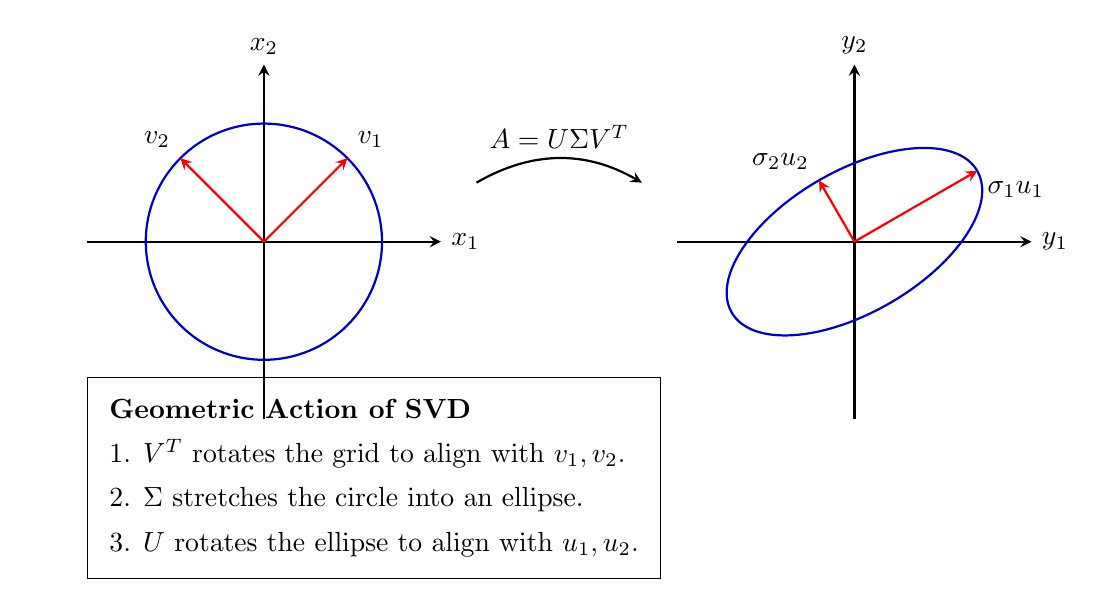
\begin{tikzpicture}[scale=1.5]
    % Background fill to ensure layering
    \fill[white] (-2,-1.5) rectangle (6,1.5);
    
    % Left side: Unit Circle
    \draw[thick, ->, >=stealth] (-1.5,0) -- (1.5,0) node[right] {$x_1$};
    \draw[thick, ->, >=stealth] (0,-1.5) -- (0,1.5) node[above] {$x_2$};
    \draw[thick, blue!80!black] (0,0) circle (1cm);
    
    \draw[thick, ->, >=stealth, red] (0,0) -- (0.707, 0.707) node[above right, black] {$v_1$};
    \draw[thick, ->, >=stealth, red] (0,0) -- (-0.707, 0.707) node[above left, black] {$v_2$};
    
    % Arrow in middle
    \draw[thick, ->, >=stealth] (1.8, 0.5) to[bend left] node[above] {$A = U \Sigma V^T$} (3.2, 0.5);
    
    % Right side: Ellipse
    \begin{scope}[shift={(5,0)}]
        \draw[thick, ->, >=stealth] (-1.5,0) -- (1.5,0) node[right] {$y_1$};
        \draw[thick, ->, >=stealth] (0,-1.5) -- (0,1.5) node[above] {$y_2$};
        
        % Draw ellipse rotated
        \draw[thick, blue!80!black, rotate=30] (0,0) ellipse (1.2cm and 0.6cm);
        
        \draw[thick, ->, >=stealth, red, rotate=30] (0,0) -- (1.2, 0) node[below right, black] {$\sigma_1 u_1$};
        \draw[thick, ->, >=stealth, red, rotate=30] (0,0) -- (0, 0.6) node[above left, black] {$\sigma_2 u_2$};
    \end{scope}
    
    % Legend
    \node[align=left, inner sep=8pt, anchor=west, draw] at (-1.5, -2) {
        \textbf{Geometric Action of SVD}\\[4pt]
        1. $V^T$ rotates the grid to align with $v_1, v_2$.\\[4pt]
        2. $\Sigma$ stretches the circle into an ellipse.\\[4pt]
        3. $U$ rotates the ellipse to align with $u_1, u_2$.
    };
\end{tikzpicture}
\end{center}

\subsection{B) Forward and Backward Links}
\textbf{Backward Links:} The SVD is the culmination of the entire linear algebra curriculum. It relies on the Spectral Theorem (symmetric matrices have real eigenvalues and orthogonal eigenvectors), the Gram-Schmidt process (for completing orthonormal bases), and the Four Fundamental Subspaces (Col A, Nul A, Row A, Nul $A^T$).

\textbf{Forward Links:} The SVD is the absolute bedrock of modern data science. It directly leads to Principal Component Analysis (PCA) in statistics. In numerical analysis, it provides the most numerically stable way to compute the rank of a matrix and solve ill-posed least-squares problems via the Moore-Penrose Pseudoinverse.

\newpage
\section{Part 6: Abstract Real-World Modeling (AI, ML, \& Quant Finance)}

\subsection{A) Concrete Scenarios}
1. \textbf{Generative AI \& NLP (Latent Semantic Analysis):} In natural language processing, a corpus of text is represented as a massive term-document matrix $A$. Applying truncated SVD to $A$ extracts the hidden "latent" concepts linking words and documents, allowing AI to understand that "car" and "automobile" are semantically identical.
2. \textbf{Quantitative Finance (Yield Curve Dynamics):} The term structure of interest rates (the yield curve) fluctuates daily. Quants use PCA (driven by SVD) on historical yield data to isolate the three primary risk factors driving the bond market: the "Level" (parallel shift), "Steepness" (slope change), and "Curvature" (butterfly shift).

\subsection{B) Model Problem Setup: Yield Curve PCA}
Let $Y \in \R^{T \times N}$ be a matrix representing daily changes in interest rates, where $T$ is the number of trading days (e.g., 252) and $N$ is the number of bond maturities (e.g., 10 tenors: 1M, 3M, 1Y, ..., 30Y). We assume the data is mean-centered.

The empirical covariance matrix of the yield changes is given by:
\[
C = \frac{1}{T-1} Y^T Y
\]
To identify the uncorrelated risk factors driving the market, we perform an SVD on the data matrix $Y$:
\[
Y = U \Sigma V^T
\]
By substitution, the covariance matrix becomes:
\[
C = \frac{1}{T-1} (U \Sigma V^T)^T (U \Sigma V^T) = \frac{1}{T-1} V \Sigma^2 V^T
\]
This is the eigenvalue decomposition of $C$. The columns of $V$ (the right singular vectors) represent the \textbf{Principal Components} (the fundamental shapes of yield curve movements). The diagonal entries of $\frac{1}{T-1}\Sigma^2$ represent the variance explained by each principal component.

In algorithmic trading, a quant will truncate this model to the first $k=3$ components (Level, Steepness, Curvature), creating a reduced-rank approximation:
\[
\hat{Y} = U_k \Sigma_k V_k^T
\]
This dramatically reduces the dimensionality of the stochastic differential equations needed to price complex interest rate derivatives, filtering out market noise while retaining 99\% of the variance.

\newpage
\section{Part 7: Common Variations and Untested Concepts}

While the homework covered the mechanics of finding the SVD, it did not explicitly test the computation of the \textbf{Moore-Penrose Pseudoinverse} ($A^+$) for solving least-squares problems, which is a critical application mentioned in the text.

\subsection{The Moore-Penrose Pseudoinverse}
If $A = U \Sigma V^T$, the pseudoinverse is defined as:
\[
A^+ = V \Sigma^+ U^T
\]
where $\Sigma^+$ is formed by taking the reciprocal of every non-zero singular value in $\Sigma$, leaving the zeros alone, and then transposing the matrix. The vector $\hat{x} = A^+ b$ provides the least-squares solution to $Ax = b$ with the minimum possible length.

\textbf{Worked Example:}
Find the pseudoinverse of $A = \begin{bmatrix} 2 & 0 \\ 0 & 0 \end{bmatrix}$ and use it to find the shortest least-squares solution to $Ax = \begin{bmatrix} 4 \\ 5 \end{bmatrix}$.

\textbf{Solution:}
From Problem 5, we know the SVD of $A$:
\[
U = \begin{bmatrix} 1 & 0 \\ 0 & 1 \end{bmatrix}, \quad \Sigma = \begin{bmatrix} 2 & 0 \\ 0 & 0 \end{bmatrix}, \quad V = \begin{bmatrix} 1 & 0 \\ 0 & 1 \end{bmatrix}
\]
\textit{(Note: We adjusted the signs from Problem 5 to make $U=I$ for simplicity, which is valid since $v_1$ can be chosen as positive).}
To find $\Sigma^+$, we invert the non-zero entries and transpose:
\[
\Sigma^+ = \begin{bmatrix} 1/2 & 0 \\ 0 & 0 \end{bmatrix}
\]
Thus, the pseudoinverse is:
\[
A^+ = V \Sigma^+ U^T = \begin{bmatrix} 1 & 0 \\ 0 & 1 \end{bmatrix} \begin{bmatrix} 1/2 & 0 \\ 0 & 0 \end{bmatrix} \begin{bmatrix} 1 & 0 \\ 0 & 1 \end{bmatrix} = \begin{bmatrix} 1/2 & 0 \\ 0 & 0 \end{bmatrix}
\]
The least squares solution is:
\[
\hat{x} = A^+ b = \begin{bmatrix} 1/2 & 0 \\ 0 & 0 \end{bmatrix} \begin{bmatrix} 4 \\ 5 \end{bmatrix} = \begin{bmatrix} 2 \\ 0 \end{bmatrix}
\]
This perfectly minimizes $\|Ax - b\|$ while keeping $\|\hat{x}\|$ as small as possible.

\newpage
\section{Part 8: Advanced Diagnostic Testing: "Find the Flaw"}

\textit{Below are five problems with complete solutions. However, each solution contains a single, subtle, yet critical flaw. Your task as the grader is to identify the error, explain why it is wrong, and provide the correct step.}

\vspace{1em}
\textbf{Problem 1:} Find the singular values of $A = \begin{bmatrix} 0 & 3 \\ 4 & 0 \end{bmatrix}$.
\textbf{Flawed Solution:}
1. $A^TA = \begin{bmatrix} 0 & 4 \\ 3 & 0 \end{bmatrix} \begin{bmatrix} 0 & 3 \\ 4 & 0 \end{bmatrix} = \begin{bmatrix} 16 & 0 \\ 0 & 9 \end{bmatrix}$.
2. The eigenvalues of $A^TA$ are $\lambda_1 = 16$ and $\lambda_2 = 9$.
3. The singular values are $\sigma_1 = 16$ and $\sigma_2 = 9$.
\textbf{Flaw:} The singular values are the \textit{square roots} of the eigenvalues, not the eigenvalues themselves.
\textbf{Correction:} $\sigma_1 = \sqrt{16} = 4$ and $\sigma_2 = \sqrt{9} = 3$.

\vspace{1em}
\textbf{Problem 2:} Construct $U$ for the SVD of $A = \begin{bmatrix} 1 & 1 \\ 0 & 0 \end{bmatrix}$.
\textbf{Flawed Solution:}
1. $A^TA = \begin{bmatrix} 1 & 1 \\ 1 & 1 \end{bmatrix}$. Eigenvalues are $\lambda_1 = 2, \lambda_2 = 0$. $\sigma_1 = \sqrt{2}$.
2. Eigenvector for $\lambda_1$ is $v_1 = \begin{bmatrix} 1 \\ 1 \end{bmatrix}$.
3. $u_1 = \frac{1}{\sigma_1} A v_1 = \frac{1}{\sqrt{2}} \begin{bmatrix} 1 & 1 \\ 0 & 0 \end{bmatrix} \begin{bmatrix} 1 \\ 1 \end{bmatrix} = \frac{1}{\sqrt{2}} \begin{bmatrix} 2 \\ 0 \end{bmatrix} = \begin{bmatrix} \sqrt{2} \\ 0 \end{bmatrix}$.
\textbf{Flaw:} The vector $v_1$ was not normalized to a unit vector before computing $u_1$.
\textbf{Correction:} $v_1$ must be $\frac{1}{\sqrt{2}}\begin{bmatrix} 1 \\ 1 \end{bmatrix}$. Then $u_1 = \frac{1}{\sqrt{2}} A v_1 = \frac{1}{\sqrt{2}} \begin{bmatrix} 1 & 1 \\ 0 & 0 \end{bmatrix} \begin{bmatrix} 1/\sqrt{2} \\ 1/\sqrt{2} \end{bmatrix} = \begin{bmatrix} 1 \\ 0 \end{bmatrix}$.

\vspace{1em}
\textbf{Problem 3:} Find the rank of $A$ if its singular values are $\sigma_1 = 5, \sigma_2 = -3, \sigma_3 = 0$.
\textbf{Flawed Solution:}
1. The rank is the number of non-zero singular values.
2. There are two non-zero singular values (5 and -3).
3. Therefore, the rank is 2.
\textbf{Flaw:} Singular values are defined as the principal square roots of eigenvalues of $A^TA$, meaning they can \textit{never} be negative. The premise of the problem contains an impossible matrix state.
\textbf{Correction:} A matrix cannot have a singular value of -3. If $\lambda = 9$, $\sigma = \sqrt{9} = 3$.

\vspace{1em}
\textbf{Problem 4:} Determine the dimensions of $U, \Sigma, V$ for a $4 \times 7$ matrix $A$.
\textbf{Flawed Solution:}
1. $U$ is an orthogonal matrix, so it must be $7 \times 7$.
2. $\Sigma$ must match the dimensions of $A$, so it is $4 \times 7$.
3. $V$ is an orthogonal matrix, so it must be $4 \times 4$.
\textbf{Flaw:} The dimensions of $U$ and $V$ are swapped. $U$ corresponds to the column space ($\R^m$), and $V$ corresponds to the row space ($\R^n$).
\textbf{Correction:} $U$ must be $m \times m = 4 \times 4$. $V$ must be $n \times n = 7 \times 7$.

\vspace{1em}
\textbf{Problem 5:} Write the SVD expansion of $A$ given $\sigma_1=2, u_1=\begin{bmatrix} 1 \\ 0 \end{bmatrix}, v_1=\begin{bmatrix} 0 \\ 1 \end{bmatrix}$.
\textbf{Flawed Solution:}
1. The spectral decomposition is $A = \sigma_1 u_1 v_1$.
2. $A = 2 \begin{bmatrix} 1 \\ 0 \end{bmatrix} \begin{bmatrix} 0 \\ 1 \end{bmatrix} = \begin{bmatrix} 0 \\ 0 \end{bmatrix}$.
\textbf{Flaw:} The expansion requires the outer product $u_1 v_1^T$, not the standard matrix multiplication of two column vectors (which is undefined/dimensionally invalid anyway).
\textbf{Correction:} $A = \sigma_1 u_1 v_1^T = 2 \begin{bmatrix} 1 \\ 0 \end{bmatrix} \begin{bmatrix} 0 & 1 \end{bmatrix} = 2 \begin{bmatrix} 0 & 1 \\ 0 & 0 \end{bmatrix} = \begin{bmatrix} 0 & 2 \\ 0 & 0 \end{bmatrix}$.

\end{document}